% Abstract for the TUM report document
% Included by MAIN.TEX


\clearemptydoublepage
\phantomsection
\addcontentsline{toc}{chapter}{Abstract}

\begin{center}
  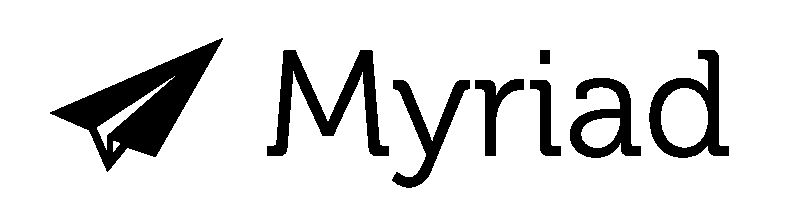
\includegraphics[height=2cm]{figures/myriad-logo.pdf}
\end{center}


\begin{center}
{\Large \bf Abstract}
\end{center}

This thesis introduces the myriad system for email mass communication.

Despite its age, Email has remained the prevalent form of electronic communication, it's usage being wildly different from how it was imagined. The tools to handle it, however, are still stuck in their original UI metaphors.

Myriad aims at producing personalised communication on a comparable level to manually composed messages, while reducing user effort.
A cross-over of mailmerge and customer support or helpdesk software, it enables managing big volumes of bidirectional email-based communication.
It is based on a self-developed framework for separating information extraction, decision making, and personalisation steps in communication, which is also introduced.

The myriad system consists of a server component that handles interfacing with email servers, a core logic system, and a web front-end for users. It includes interoperability with Google Docs' Spreadsheets and Google Mail Labels. \\ It can be accessed at \url{http://myriad.ludwigschubert.de}.

\begin{center}
{\Large \bf Classification}
\end{center}

\textbf{ACM:} Human-centered computing $\rangle$ Human computer interaction (HCI) $\rangle$ Interaction paradigms $\rangle$ Collaborative interaction

\textbf{General Terms:} Design, Human Factors, Experimentation

\textbf{Keywords:} Email, Workflow, Helpdesk, Mail merge, Crowdsourcing, Personalised Communication, Assisted Templating, Generated Documents, Web-Application
